\subsubsection{Atender Solicitud}
En en siguiente diagrama\ref{fig:Diagrama de Secuencia - Visualizar Solicitudes de Refaccion} se muestra la secuencia que corresponde a la atención de todas las solicitudes que los diversos empleados han realizado para que puedan hacer su trabajo, al momento de aceptar la solicitud y atenderla el administrador ingresará unos datos que el sistema solicite, estos datos tendrán que ser verificados:
\begin{itemize}
	\item \textbf{Datos válidos:} Los datos ingresados por el administrador son correctos y cuentan con el formato específico para ser ingresados a la base de datos y atender a la solicitud del empleado.  
	\item \textbf{Datos no válidos} Los datos ingresados no son correctos o no cumplen con las especificaciones de formato.
\end{itemize}
\begin{figure}[!h]
	\centering
	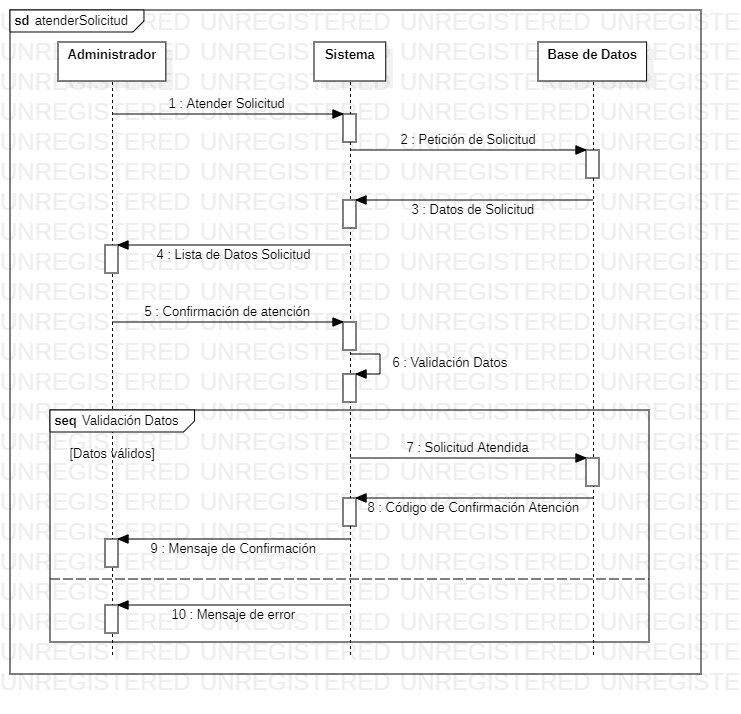
\includegraphics[width=0.8\textwidth]{./diseno/vprocesos/imagenes/atenderSolicitud}
	\caption{Diagrama de Secuencia - Atender Solicitud de Refacción}
	\label{fig:Diagrama de Secuencia - Atender Solicitud de Refaccion}
\end{figure}
\clearpage